\documentclass[12pt, a4paper]{article}
\usepackage [ngerman]{babel}
\usepackage[utf8]{inputenc}
\usepackage[T1]{fontenc}
%\renewcommand{\rmdefault}{phv} % Arial
%\renewcommand{\sfdefault}{phv} % Arial
\usepackage{color}
\usepackage{fancyhdr}
\usepackage{graphicx}
\usepackage{float}
\usepackage{geometry}
\usepackage[table]{xcolor}
\usepackage{helvet}

\parindent0em

%Inhaltsverzeichnis mit Links füllen
\usepackage{hyperref}
\hypersetup{
    colorlinks,
    citecolor=black,
    filecolor=black,
    linkcolor=black,
    urlcolor=black
}

\setlength{\fboxsep}{0pt} %Padding: Bilderrahmen
\setlength{\fboxrule}{2pt} %Breite: Bilderrahmen
\setlength{\arrayrulewidth}{0.7pt} %Breite: Tabellenrahmen
\usepackage[font=small,skip=3pt]{caption}

\geometry{verbose,a4paper,bmargin=30mm,lmargin=25mm,rmargin=20mm}

\pagestyle{fancy} %eigener Seitenstil
\fancyhf{} %alle Kopf- und Fußzeilenfelder bereinigen
\fancyhead[L]{Programmieren 3} %Kopfzeile links
\fancyhead[C]{Robin Hake \\ Benedikt Brüntrup} %zentrierte Kopfzeile
\fancyhead[R]{
\includegraphics[width=4cm]{Bilder/HS_OWL_RGB_Rot.jpg}} %Kopfzeile rechts
\renewcommand{\headrulewidth}{0.4pt} %obere Trennlinie
\fancyfoot[C]{\thepage} %Seitennummer
\renewcommand{\footrulewidth}{0.4pt} %untere Trennlinie


%Farben
\definecolor{Grau}{gray}{0.3}
\definecolor{Hellgrau}{gray}{0.8}


\begin{document}


\begin{titlepage}
Hochschule Ostwestfalen-Lippe \\
Fachbereich 8 - Umweltingeneurwesen und Angewandte Informatik \\
Fachgebiet Angewandte Informatik \\
Programmieren 3 \\
5. Semester WS 2015/16\\
\vspace{2cm}

\begin{center}
\begin{Large}
\textbf{Dokumentation} \\
\end{Large}
\vspace{2cm}

\begin{Large}
\textbf {Implementierung eines Prototypen für eine Verwaltungssoftware für ein Call-Center} \\[0.35cm]
\end{Large}
Von \\[0.35cm]
Robin Hake \\
15306070 \\[0.35cm]
und\\[0.35cm]
Benedikt Brüntrup \\
15306067 \\[0.35cm]
\end{center}

\vfill
Erstprüfer: Prof. Dr. Ralf Hesse \\
Eingereicht am: {\today}
\end{titlepage}

\newpage
\tableofcontents


\vfill
\newpage


\section{Aufgabenstellung}
Als Abschlussarbeit des Moduls \glqq Programmiersprachen 3\grqq{} sieht die Prüfungsordnung die Abgabe eines in JavaEE implementierten Software-Projekts vor. Hierzu ist von den Professor Ralf Hesse eine Liste mit möglichen Abschlussthemen bereitgestellt worden. Von dieser Liste sollte sich ein Thema ausgesucht werden und zwei Anwendungsszenarien des Themas in einen Software-Prototyp umgesetzt werden. Der Software-Prototyp ist dabei auf Basis eines dreischichtigen Ansatz umzusetzen.  Die Gruppe Robin Hake und Benedikt Brüntrup entschloss sich das Thema \glqq Verwaltungssoftware für ein Call-Center\grqq{} umzusetzen.

\section{Projektplanung}
Dieser Abschnitt beschreibt, wie bei der Projektplanung vorgegangen wurde. Es wird auf die  Anforderungsanalyse, den ersten Designentwurf, den Datenbankentwurf und das gewählte Entwurfsmuster eingegangen.

\subsection{Anforderungsanalyse}
Zu Beginn der Projektplanung wurde mit Hilfe eines Use-Case-Diagramms ermittelt was das Projekt alles können soll. Die Ermittlungen haben ergeben, dass es einen Administrator und Standardbenutzer geben soll. Der Administrator soll Benutzer verwalten können und die Standardbenutzer sollen mit Tickets arbeiten können. Genauere Details zur Anforderungsanalyse kann den Use-Case-Diagramm der \textit{Abbildung 1} entnommen werden.

\begin{figure}[H]
	\begin{center}
	%\fcolorbox{Grau}{black}{
	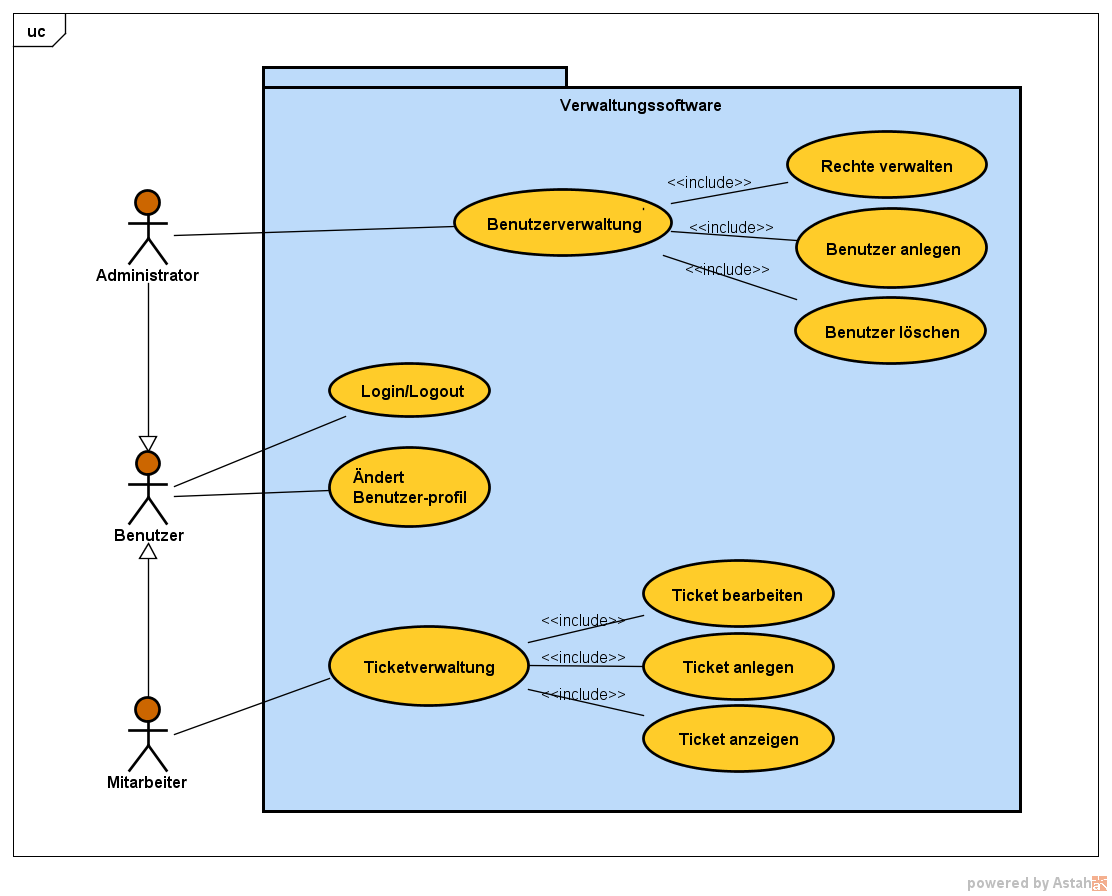
\includegraphics[width=110mm]{Bilder/UseCaseAnforderungsanalyse.png}
	%}
	\end{center}
	\caption{Anforderungsanalyse als Use-Case-Diagramm}
\end{figure}

\subsection{Erster Designentwurf}

Als nächstes wurde mit dem Programm PowerPoint ein erster Designentwurf für die Weboberfläche des Projektes entworfen. Hierbei wurde sich für ein fensterbasiertes Design entschlossen. Dieses bietet den Vorteil, dass das Projekt einfach erweitert werden kann. Soll das Software-Produkt eine neue Funktion haben kann einfach ein neues Fenster hinzugefügt werden. Die folgende Abbildung zeigt den ersten Designentwurf in PowerPoint.

\begin{figure}[H]
	\begin{center}
		\fcolorbox{Grau}{Grau}{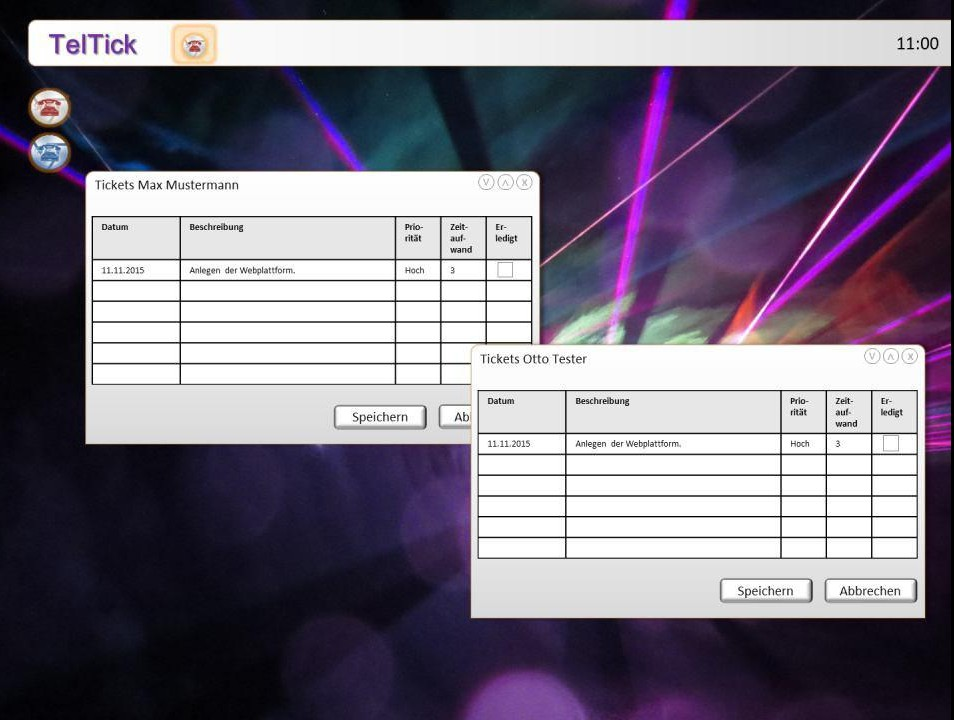
\includegraphics[width=98mm]{Bilder/designentwurf.jpg}}
	\end{center}
	\caption{Erster Designentwurf in PowerPoint}
\end{figure}

\subsection{Datenbankentwurf}
Nachdem das grundlegende Design der Webseite festgelegt worden war, wurde sich über die Datenhaltung Gedanken gemacht. Es wurde ermittelt welche Daten das Software-Projekt persistent speichern soll und wie diese Daten im Zusammenhang stehen. Aus dieser Erkenntnis wurde die in der \textit{Abbildung 3} gezeigte Datenbankstruktur festgelegt.

Die \textit{Tabelle 1} beschreibt wofür welche Relation in der Datenbank benötigt wird.
\begin{table}[H]
	\begin{center}
		\begin{tabular}{|p{3cm}|p{10cm}|}
			\hline 
				\cellcolor{Hellgrau}Tabellenname & \cellcolor{Hellgrau}Beschreibung \\ 
			\hline 
				Mitarbeiter & In dieser Relation werden die Mitarbeiter hinterlegt, die sich an der Webseite anmelden können sollen.\\ 
			\hline
				Rechte & In dieser Relation werden die Fenster eingetragen, auf die ein bestimmter Mitarbeiter Zugriffsrechte haben soll.\\ 
			\hline
				Ticket & Enthält die erstellten Tickets.\\ 
			\hline
				Fenster & Enthält die Abmaße, die Titel und die Pfade zun den JSP-Dateien der Fenster, die auf der Webseite angezeigt werden sollen.\\ 
			\hline
				Ticketzuweisung & Weißt ein Ticket einen bestimmten Benutzer zu.\\ 
			\hline
		\end{tabular}
	\end{center}
	\caption{Beschreibung der einzelnen Relationen}
\end{table}

\begin{figure}[H]
	\begin{center}
		%\fcolorbox{Grau}{Grau}{
		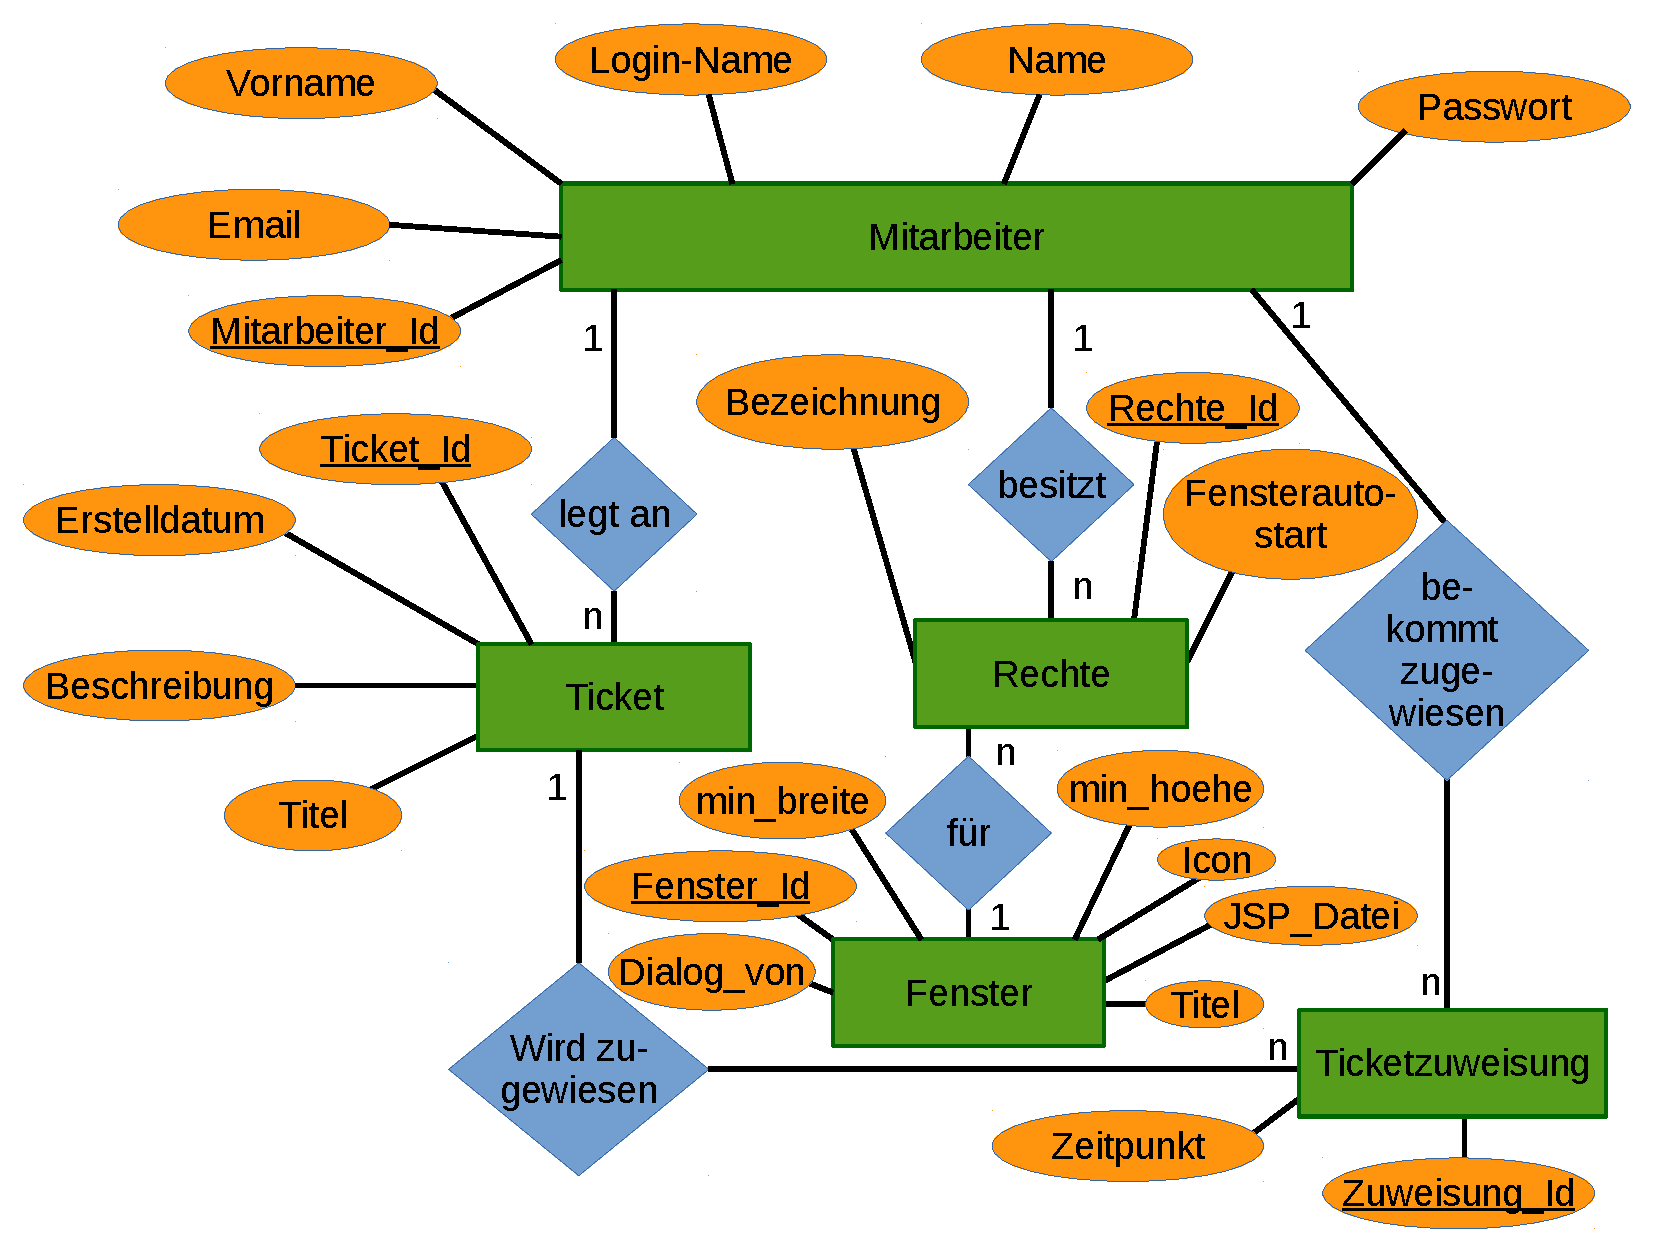
\includegraphics[width=120mm]{Bilder/erd.pdf}
		%}
	\end{center}
	\caption{Datenbankstruktur}
\end{figure}

\subsection{Architektur}
Als Architektur-Modell wurde das MVC-Modell (\textbf{M}odel, \textbf{V}iew, \textbf{C}ontrol) gewählt. Hierbei handelt es sich, wie in der Aufgabenstellung erwünscht, um ein Dreischichtenmodell. Das Use-Case-Diagramm der \textit{Abbildung 4} beschreibt wofür genau welche Schicht zuständig ist.

\begin{figure}[H]
	\begin{center}
		%\fcolorbox{Grau}{Grau}{
		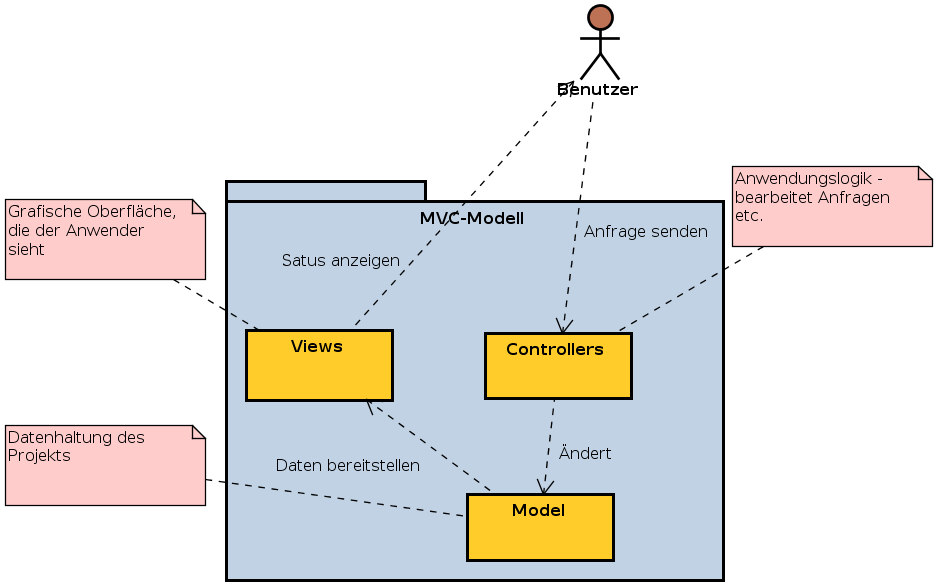
\includegraphics[width=130mm]{Bilder/MVC-Modell.png}
		%}
	\end{center}
	\caption{MVC-Modell}
\end{figure}

Die \textit{Abbildung 5} stellt da, wie das MVC-Modell beim Projekt umgesetzt wurde. Die \glqq Views\grqq{} wurden im Projekt durch JSP-Seiten umgesetzt, die \glqq Controllers\grqq{} durch Servlets und das \glqq Model\grqq{} durch DAO-Objekte. Diese DAO-Objekte mappen die Datenbank in normale Java-Objekte, sodass der Anwendungsentwickler wie gewohnt mit Java-Klassen arbeiten kann und nicht im Quellcode direkt Datenbankabfragen senden muss. Dafür bieten die DAO-Objekte einfache \glqq Store\grqq{}- und \glqq Load\grqq{}-Methoden. Diese Methoden mappen ein Java-Objekt dann in der Datenbank. 
\begin{figure}[H]
	\begin{center}
		%\fcolorbox{Grau}{Grau}{
		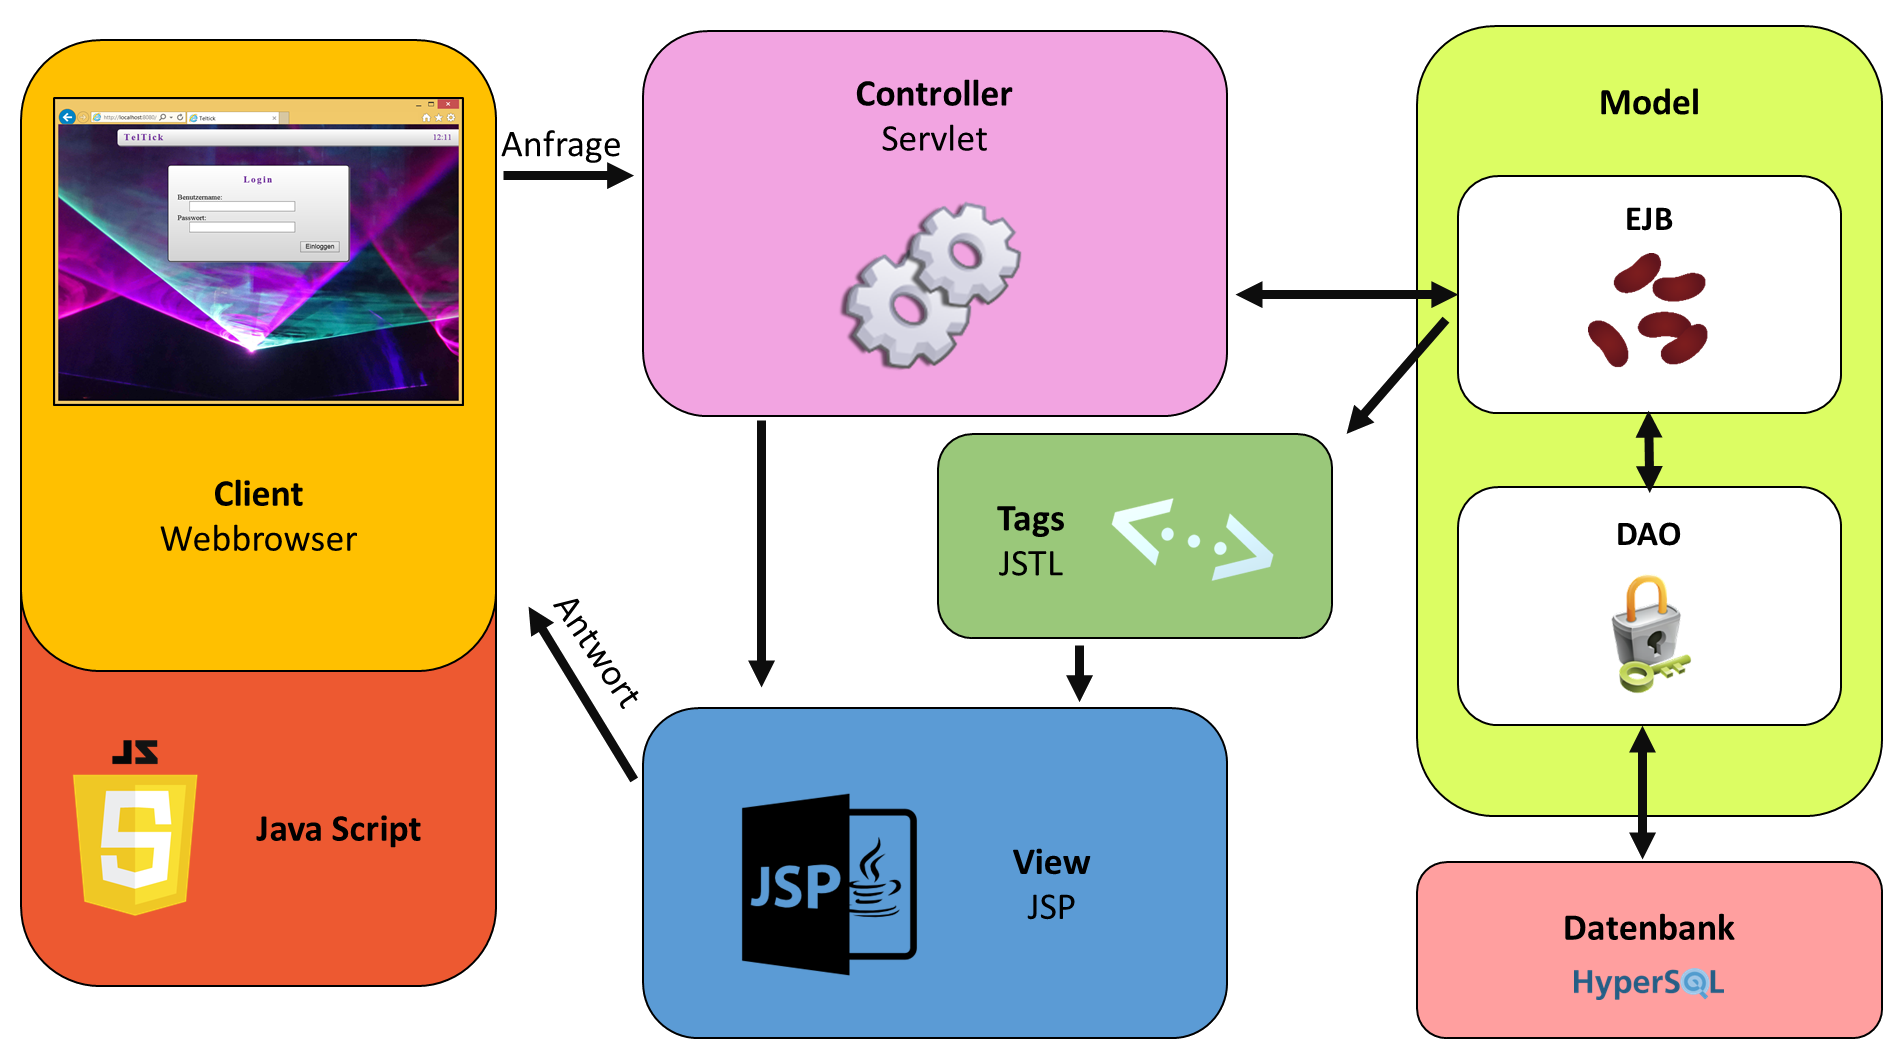
\includegraphics[width=130mm]{Bilder/archDiagramm.png}
		%}
	\end{center}
	\caption{Architektur des Projektes}
\end{figure}

\subsection{Der Desktopansatz}
Beim Projekt wurde sich entschlossen ein Desktop-Fenster-Ansatz zu benutzen, da dieses eine gute Möglichkeit ist ein Projekt möglich erweiterbar zu programmieren. Es bietet die Möglichkeit ein Projekt modular erweiterbar zu gestalten. Soll eine neues Modul zum Projekt hinzugefügt werden muss nur auf den Desktop ein neues Icon hinzugefügt werden, welches ein Fenster mit den neuen Module öffnet. Somit können Module auch problemlos ausgetauscht werden.


\section{Implementierung}
In diesem Abschnitt wird beschrieben, wie Einzelheiten des Projekts in JavaEE umgesetzt wurden. Es wird auf den Desktop-Aufbau und der Umsetzung der ausgewählten USE-Cases eingegangen.

\subsection{Umsetzung des Desktops}
Der Desktop besteht, wie in der \textit{Abbildung 7} gezeigt aus mehreren verschachtelten JSP-Dateien. Nach dem Anmelden wird standardmäßig nur die \glqq desktop.jsp\grqq{} geladen. Die Verschaltung wird erstellt wenn der Benutzer, wie bei \textit{Abbildung 6} ein neues Fenster öffnet.

\begin{figure}[H]
	\begin{center}
		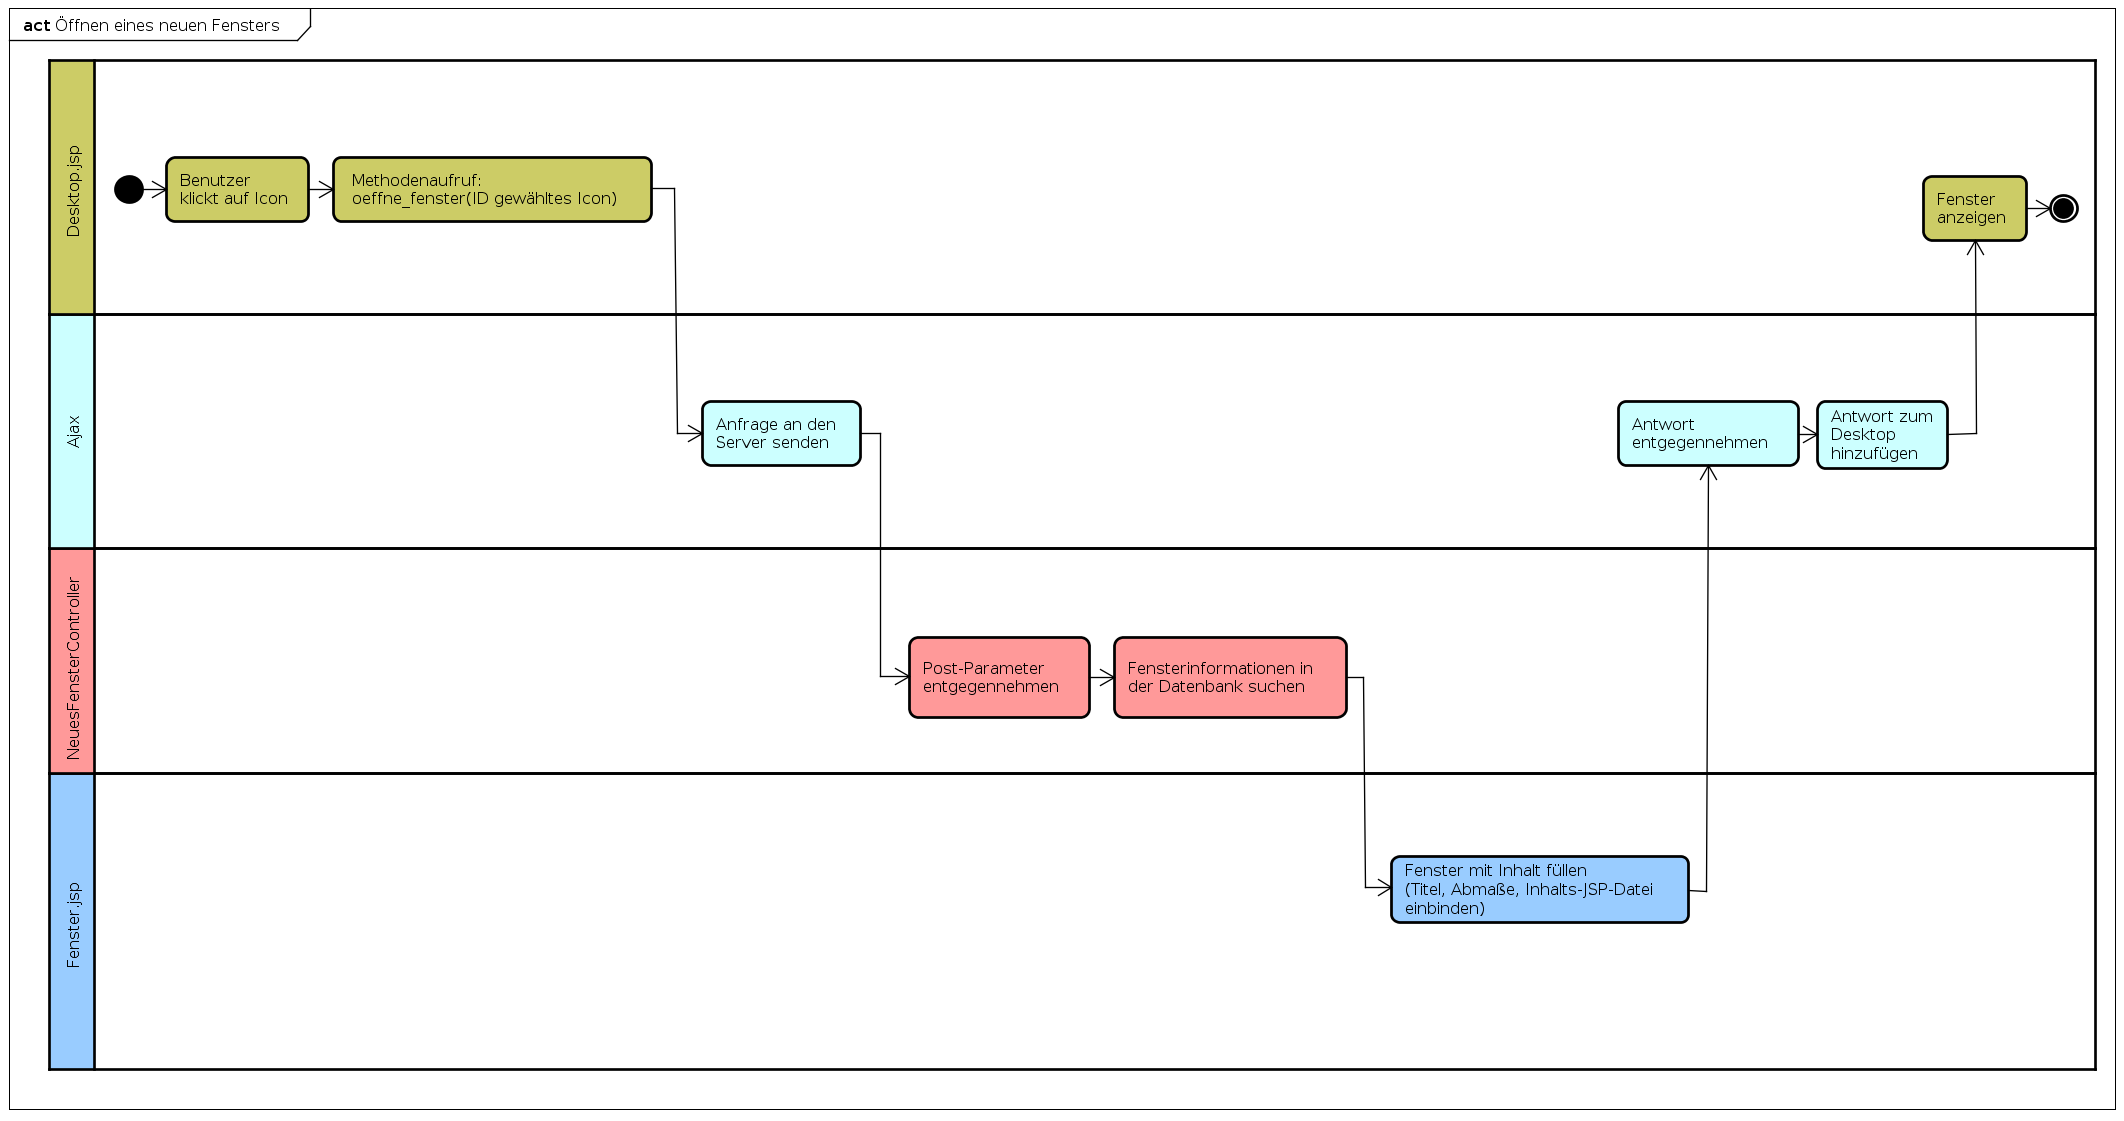
\includegraphics[width=220mm,angle=90]{Bilder/fenster_oeffnen.png}
	\end{center}
	\caption{Öffnen eines neuen Fensters}
\end{figure}

\begin{figure}[H]
	\begin{center}
		%\fcolorbox{Grau}{Grau}{
		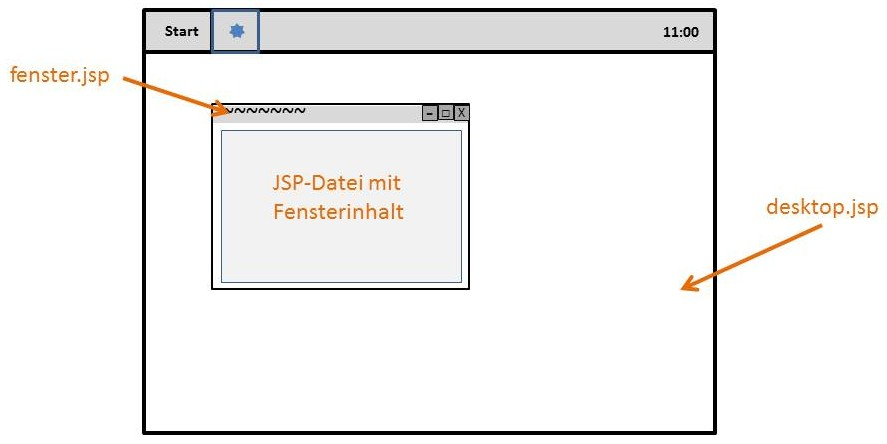
\includegraphics[width=110mm]{Bilder/desktop.jpg}
		%}
	\end{center}
	\caption{Aufbau des Desktops}
\end{figure}





%\section{Literaturverzeichnis}

%\subsection*{Literatur}

%\textsc{Felinto, D. $ \& $ Pan, M} (2013): \textit{Game Development with Blender} - Cengage Delmar
%\\
%\subsection*{Onlinequellen}
%\begin{itemize}
%	\item \url{http://www.blenderhilfe.de}
%	\item \url{http://www.blender.org}
%	\item \url{https://de.wikibooks.org/wiki/Blender_Dokumentation}
%\end{itemize}

\end{document}